\documentclass[aps,prl, reprint]{revtex4-2}
%\usepackage[margin=0.5in]{geometry} 
\usepackage{graphicx}% Include figure files
\usepackage{dcolumn}% Align table columns on decimal point
%\usepackage{bm}% bold math
%\usepackage[mathlines]{lineno}% Enable numbering of text and display math
%\usepackage{hyperref}% add hypertext capabilities
%\usepackage{relsize}
%\usepackage[usenames,dvipsnames,svgnames,table]{xcolor}
%\usepackage{proofread}
%\newcommand{\bd}[1] {\frac{#1}{b}}
%\usepackage{comment}
%\usepackage{amsmath,amsthm,amssymb,scrextend}
\usepackage{physics, qcircuit}
\usepackage{breqn}
%\usepackage{url}
\usepackage{natbib, courier}
\bibliographystyle{apsrev4-2}


\begin{document}
\title{Simulating the Heisenberg Model}
\date{\today}
\author{Timothy Skaras}
\affiliation{Department of Physics$,$ Cornell University$,$ Ithaca$,$ New York$,$ 14853}
\begin{abstract}
We estimate the entanglement entropy of the GHZ state using both simulated and real measurement data. We use Qiskit to measure the target state in the Pauli basis and then use the classical shadows protocol to estimate the entanglement entropy from our measurement data. Our estimated value aligns very well with theory for our simulated data (relative error $\leq 0.15\%$), but our estimated value based on real data differs substantially from the theoretical value for our target state (relative error $\approx 20\%$). We conclude that the device's large error is most likely caused by noise.
\end{abstract}

\maketitle

\section{Introduction}

\section{Experimental Hardware}

For our simulation task we will be using the \texttt{ibmq\_jakarta} device. This is a 7 qubit quantum computer that whose qubits are connected as depicted in figure \ref{fig:JakartaConnect}. Our simulation task will require us to use gates on this device, but like many other devices \texttt{ibmq\_jakarta} has a limited gate set. This means that any gate we want to execute on the device must either be in the gate set or must be broken down into the composition of gates in the gate set. The gate set on this device consists of $R_z(\theta)$; $X$, $\sqrt{X}$, and $CNOT$ gates. The first gate $R_z(\theta)$ is an arbitrary single qubit rotation about the z-axis. The second is the $\sigma^{x}$ or NOT gate. The third $\sqrt{X}$ is the square root of the NOT gate, and the last $CNOT$ is the controlled not gate. We note that $\sqrt{X}$ is equivalent (differs only by a global phase) to a $\pi/2$ rotation about the x-axis $R_x(\pi/2)$.

\begin{figure}
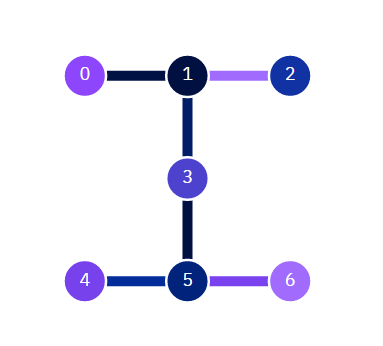
\includegraphics[width=0.4\textwidth]{JakartaDiagram.png}
\caption{This figure depicts how the qubits of the \texttt{ibmq\_jakarta} device are connected to one another. Two qubit gates can only be performed on connected qubits.}
\label{fig:JakartaConnect}
\end{figure}

\section{Quantum Simulation}

The Heisenberg model, in its most general form, is defined as
\begin{equation}
H =- \sum_{j=1}^{N}\left(J_{x} \sigma_{j}^{x} \sigma_{j+1}^{x}+J_{y} \sigma_{j}^{y} \sigma_{j+1}^{y}+J_{z} \sigma_{j}^{z} \sigma_{j+1}^{z}+h \sigma_{j}^{z}\right),
\end{equation}
where $h$ is the external magnetic field and $J_x$, $J_y$, and $J_z$ are the couplings along the x, y, and z directions respectively. The subscript $j$ denotes the site that each spin operator is acting on, and $\sigma$'s are the pauli matrices which are given by 
\begin{equation}
\begin{array}{c}
\sigma^{x}=\left(\begin{array}{cc}
0 & 1 \\
1 & 0
\end{array}\right), \,
\sigma^{y}=\left(\begin{array}{cc}
0 & -i \\
i & 0
\end{array}\right),\,
\sigma^{z}=\left(\begin{array}{cc}
1 & 0 \\
0 & -1
\end{array}\right)
\end{array}
\end{equation}
when written in the z-basis. We will be considering the XXX Heisenberg model where $J = J_x = J_y = J_z$ and $h =0$. 

The Heisenberg model is useful for studying the studying the dynamics and behavior of quantum mechanical magnetic interactions of spins. We will be simulating the quantum mechanical version of the Heisenberg model on three spin-$\frac{1}{2}$ particles. For our task, we start with the initial condition
\begin{equation}
\ket{\psi(t=0)} = \ket{110}
\end{equation}
with open boundary conditions and seek to simulate a total amount of time $\tau = \pi$. Theoretically, the time evolution of this initial condition is determined by the time-evolution operator
\begin{equation}
\ket{\psi(t=\tau)} = e^{-i \hat{H} \tau}\ket{\psi(0)},
\end{equation}
so for our problem the time evolution operator is the exponential of a sum of pauli strings. For instance, we could generically write the hamiltonian as
\begin{equation}
H = \sum_i h_i
\end{equation}
where each of the $h_i$'s is the tensor product of two pauli matrices on two nearest neighbor sites. It is fairly straightforward to implement the unitary evolution of each $h_i$ taken individually. For instance, suppose we wanted to implement
\begin{equation}
e^{-i \sigma^{z}_1 \otimes \sigma^{z}_2 t}.
\label{eqn:rzz}
\end{equation}
Our native gate set lets us do single-qubit z-rotations which are defined as
\begin{equation}
R_{z}(2t)=e^{-i \sigma^{z}_1 \otimes I t },
\end{equation}
where the identity is made explicit for clarity. We can turn this into a two qubit rotation by noticing that a $Z$ gate with a CNOT on either side is equivalent to a Z gate on two qubits, i.e., CNOT $(\sigma^{z} \otimes I)$ CNOT = $\sigma^{z} \otimes \sigma^{z}$. This relationship still holds when $\sigma^{z} \otimes I$ is in an exponential (see figure \ref{fig:JakartaConnect}). 
\begin{figure}
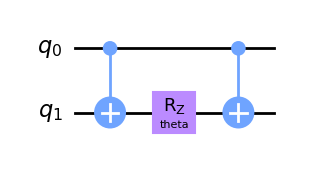
\includegraphics[width=0.35\textwidth]{Rzz.png}
\caption{This circuit shows a z-rotation sandwiched between two CNOT gates. This circuit is equivalent to the two qubit rotation given in equation (\ref{eqn:rzz}).}
\label{fig:rzz}
\end{figure}
Additionally, by using the Hadamard gate $H$ and the phase gate $S$ we can exploit relationships such as $HZH = X$ and $S X S^{\dagger}=Y$ to build other unitaries generated by individual $h_i$. This is not sufficient, however. The different $h_i$ do not commute, so we cannot split the exponential of the sum into the product of exponentials. It is for this reason that we must use a technique known as trotterization.



The challenge of quantum simulation is to find a way to implement a time evolution operator given the real-world constraints of a limited gate set and connectivity.

To get around these problems use a technique known as trotterization. 

\section{Simulation Results}

\section{Ibmq Jakarta Results}

\section{Conclusion}

\bibliography{QiskitReportBib}

\end{document}